%% exemple of a matrix/matrix product in hmat
\begin{center}
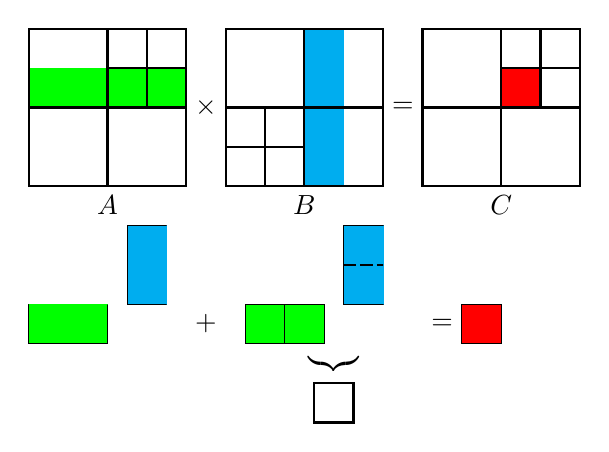
\begin{tikzpicture}[scale=0.5]
  %% matrix A
  \filldraw[fill=green, draw=green] (0,2) rectangle (2,3);
  \filldraw[fill=green, draw=green] (2,2) rectangle (3,3);
  \filldraw[fill=green, draw=green] (3,2) rectangle (4,3);
  
  \draw[ thick] (0,0) rectangle (4.0,4.0);
  \draw[ thick] (0,0) rectangle (2.0,2.0);
  \draw[ thick] (2.0,2.0) rectangle (4.0,4.0);
    \draw[ thick] (2.0,2.0) rectangle (3.0,3.0);
    \draw[ thick] (3.0,3.0) rectangle (4.0,4.0);
    \draw[ thick] (2.0,4.0) rectangle (3.0,3.0);
    \draw[ thick] (3.0,3.0) rectangle (4.0,2.0);
  \draw[ thick] (0,4.0) rectangle (2.0,2.0);
  \draw[ thick] (2.0,2.0) rectangle (4.0,0.0);

  %% matrix B
  \filldraw[fill=cyan, draw=cyan] (7.0,2.0) rectangle (8.0,4.0);
  \filldraw[fill=cyan, draw=cyan] (7.0,0.0) rectangle (8.0,2.0);
  \draw[ thick] (5.0,0) rectangle (9.0,4.0);
  \draw[ thick] (5.0,0) rectangle (7.0,2.0);
    \draw[ thick] (5.0,0) rectangle (6.0,1.0);
    \draw[ thick] (6.0,1.0) rectangle (7.0,2.0);
    \draw[ thick] (7.0,0) rectangle (6.0,1.0);
    \draw[ thick] (6.0,1.0) rectangle (5.0,0.0);
  \draw[ thick] (7.0,2.0) rectangle (9.0,4.0);
  \draw[ thick] (5,4.0) rectangle (7.0,2.0);
  \draw[ thick] (7.0,2.0) rectangle (9.0,0.0);

  %% matrix C
  \draw[thick] (10.0,0) rectangle (14.0,4.0);
  \draw[thick] (10.0,0) rectangle (12.0,2.0);
  \draw[thick] (12.0,2.0) rectangle (14.0,4.0);
    \draw[thick] (12.0,2.0) rectangle (13.0,3.0);
      \filldraw[fill=red, draw=black] (12.0,2.0) rectangle (13.0,3.0);
    \draw[thick] (13.0,3.0) rectangle (14.0,4.0);
    \draw[thick] (12.0,4.0) rectangle (13.0,3.0);
    \draw[thick] (13.0,3.0) rectangle (14.0,2.0);
  \draw[thick] (10.0,4.0) rectangle (12.0,2.0);
  \draw[thick] (12.0,2.0) rectangle (14.0,0.0);

  %% A
  \node at (4.5,2.0) {$\times$};
  \node at (9.5,2.0) {$=$};
  \node[below] at (12.0,0.0) {$C$};
  \node[below] at (7.0,0.0) {$B$};
  \node[below] at (2.0,0.0) {$A$};

  \filldraw[fill=cyan, draw=black] (8.0,-3.0) rectangle (9.0,-1.0);
  \draw[cyan] (9.0,-3.0) rectangle (9.0,-1.0);
  \draw[dashed] (8.0,-2.0) rectangle (9.0,-2.0);

  \node at (4.5,-3.5) {$+$};
  \node[below] at (7.75,-4) {$\underbrace{}$};

  \node at (10.5,-3.5) {$=$};
  \filldraw[fill=red, draw=black] (11.0,-4.0) rectangle (12.0,-3.0);
  \draw[thick] (7.25,-6.0) rectangle (8.25,-5.0);


  \filldraw[fill=green, draw=black] (0,-4) rectangle (2,-3);
  \draw[fill=green, draw=black] (0,-4) rectangle (2,-3);
  \draw[green] (0,-3) rectangle (2,-3);
  \filldraw[fill=cyan, draw=black] (2.5,-3.0) rectangle (3.5,-1.0);
  \draw[draw=cyan] (3.5,-3.0) rectangle (3.5,-1.0);

  \filldraw[fill=green, draw=black] (5.5,-4) rectangle (6.5,-3);
  \filldraw[fill=green, draw=black] (6.5,-4) rectangle (7.5,-3);

\end{tikzpicture}
\end{center}

